\chapter{移动平台设计和制造}
\label{cha:Platform}

\section{平台设计初始思路}
形式:

每个小车为一个数据点,在1-3维坐标系内动态运动(如果和ShapeBots\cite{suzuki2019shapebots}一样具备升降平台或者和SwarmOS一样具备可变色LED点阵则可以进行三维变量显示)

也可以每个小车作为一个通信节点(在电力市场的应用场景下是一个机组节点),用屏幕/位置/RGB颜色/高度直观的显示迭代的过程。

即插即用的实现:放入/取出小车,新的迭代随即开始。

\section{仿真}

Swarm仿真参考ShapeBots\cite{suzuki2019shapebots}的仿真方法\footnote{\href{https://ryosuzuki.github.io/shapebots-simulator/}{https://ryosuzuki.github.io/shapebots-simulator/}},使用Javascript在网页端编写了相应的仿真程序,进行指定数量的集群小车对于SVG格式图片的渲染和给定数据折线图或条形图的可视化绘制。

\section{定位方法}

% 如果直接插入一页PDF用
% 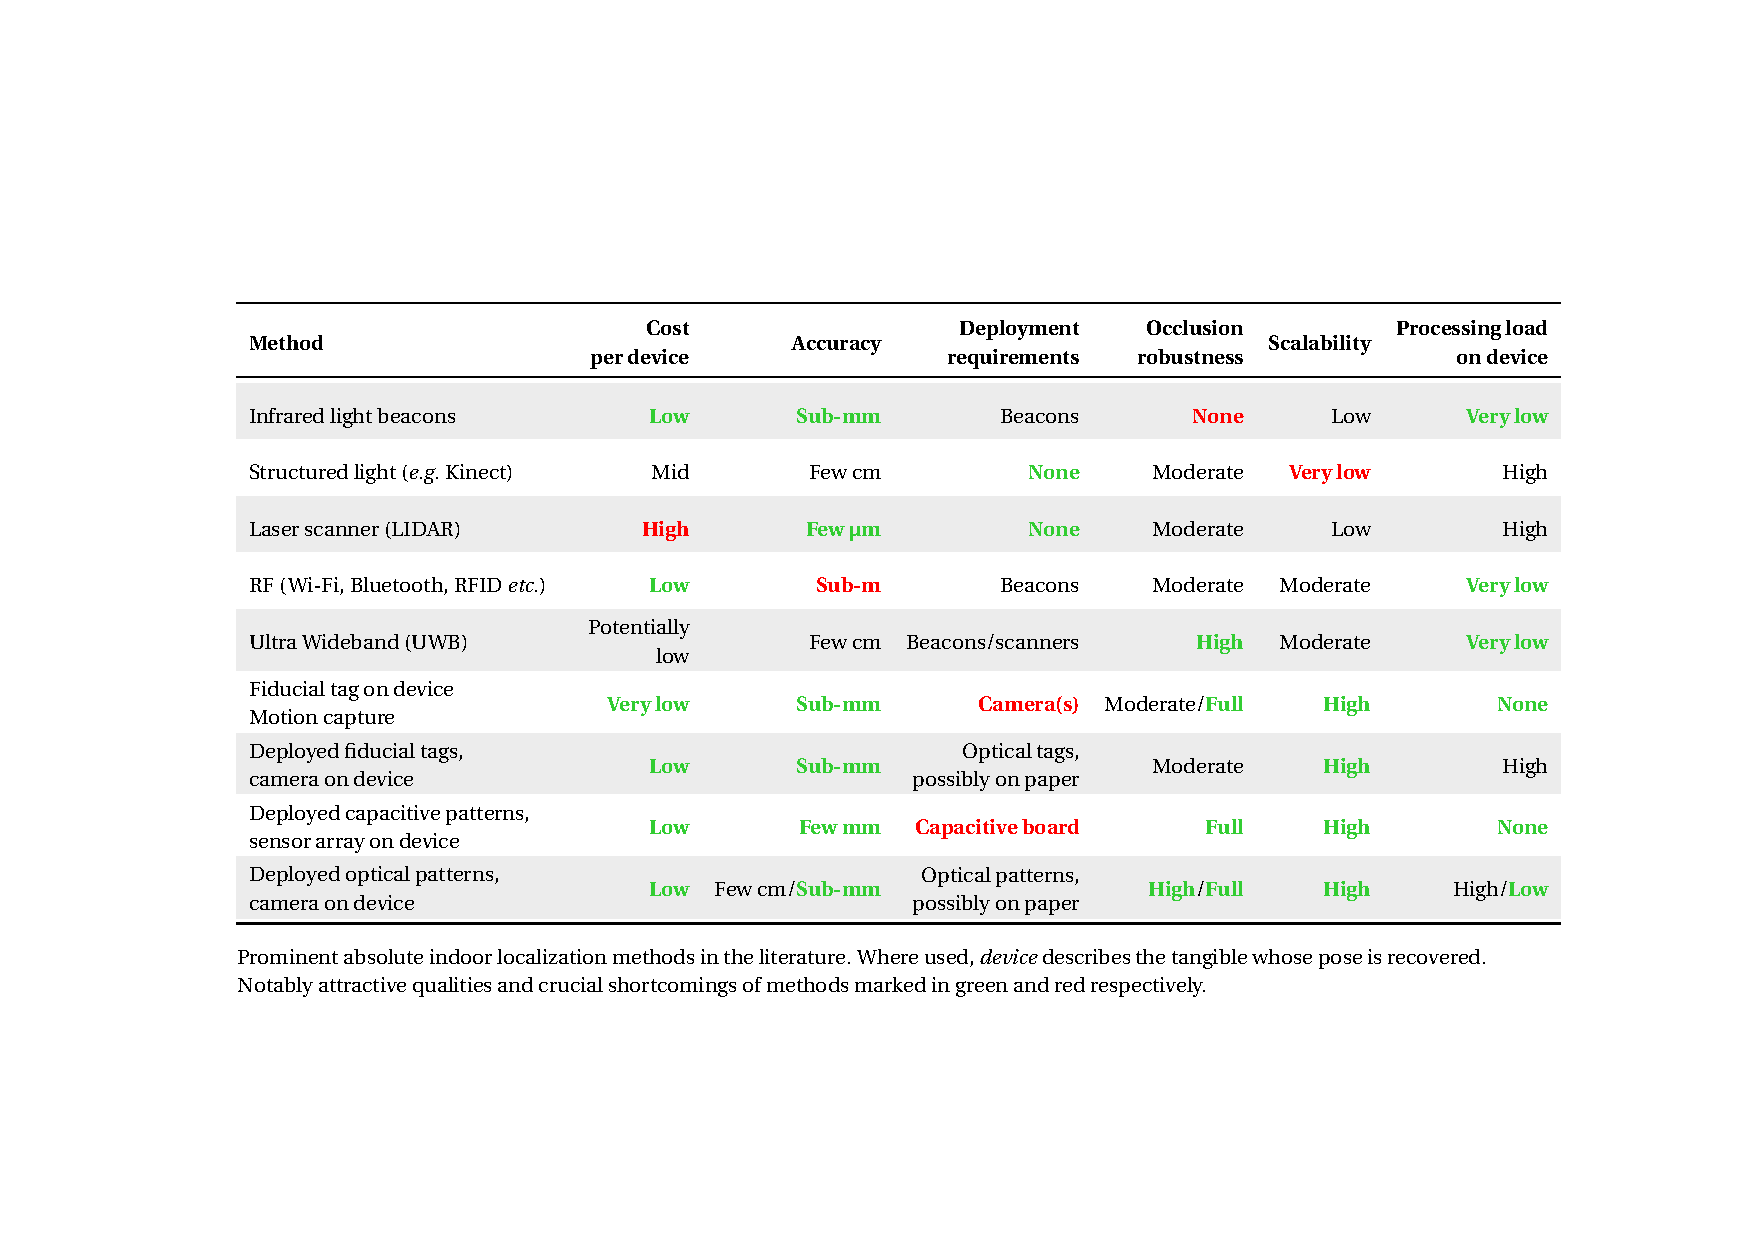
\includepdf{Prominent-absolute-indoor-localization-methods-comparison.pdf} 

% Please add the following required packages to your document preamble:
% \usepackage[table,xcdraw]{xcolor}
% If you use beamer only pass "xcolor=table" option, i.e. \documentclass[xcolor=table]{beamer}
% \usepackage{lscape}
\begin{landscape}
    \begin{table}[]
    \centering
    \begin{tabular}{lllllll}
    \hline
    Method                                                                                         & Cost per device & Accuracy      & \begin{tabular}[c]{@{}l@{}}Deployment\\ requirements\end{tabular}             & \begin{tabular}[c]{@{}l@{}}Occlusion\\ robustness\end{tabular} & Scalabiity & \begin{tabular}[c]{@{}l@{}}Processing load\\ on device\end{tabular} \\ \hline
    \rowcolor[HTML]{EFEFEF} 
    Infrared light beacons                                                                         & Low             & Sub-mm        & Beacons                                                                       & None                                                           & Low        & Very low                                                            \\
    Structured light (e.g. Kinect)                                                                 & Mid             & Few cm        & None                                                                          & Moderate                                                       & Very low   & High                                                                \\
    \rowcolor[HTML]{EFEFEF} 
    Laser scanner (LIDAR)                                                                          & High            & Few µm        & None                                                                          & Moderate                                                       & Low        & High                                                                \\
    \begin{tabular}[c]{@{}l@{}}RF (Wi-Fi, \\ Bluetooth, RFID etc.)\end{tabular}                    & Low             & Sub-m         & Beacons                                                                       & Moderate                                                       & Moderate   & Very low                                                            \\
    \rowcolor[HTML]{EFEFEF} 
    \begin{tabular}[c]{@{}l@{}}Ultra Wideband \\ (UWB)\end{tabular}                                & Potentially low & Few cm        & Beacons/scanners                                                              & High                                                           & Moderate   & Very low                                                            \\
    \begin{tabular}[c]{@{}l@{}}Fiducial tag on device\\ Motion capture\end{tabular}                & Very low        & Sub-mm        & Camera(s)                                                                     & Moderate/Full                                                  & High       & None                                                                \\
    \rowcolor[HTML]{EFEFEF} 
    \begin{tabular}[c]{@{}l@{}}Deployed fiducial tags,\\ camera on device\end{tabular}             & Low             & Sub-mm        & \begin{tabular}[c]{@{}l@{}}Optical tags, \\ possibly on paper\end{tabular}    & Moderate                                                       & High       & High                                                                \\
    \begin{tabular}[c]{@{}l@{}}Deployed capacitive patterns,\\ sensor array on device\end{tabular} & Low             & Few mm        & Capacitive board                                                              & Full                                                           & High       & None                                                                \\
    \rowcolor[HTML]{EFEFEF} 
    \begin{tabular}[c]{@{}l@{}}Deployed optical patterns,\\ camera on device\end{tabular}          & Low             & Few cm/Sub-mm & \begin{tabular}[c]{@{}l@{}}Optical patterns,\\ possibly on paper\end{tabular} & High/Full                                                      & High       & High/Low                                                            \\ \hline
    \end{tabular}
    \caption{Prominent absolute indoor localization methods in the literature. Where used, device describes the tangible whose pose is recovered. }
    \label{tab:localization}
    \end{table}
\end{landscape}

各类定位方法优缺点\cite{ozgur2018cellulo}如表~\ref{tab:localization}所示。

\section{底盘}
考虑到交互过程中需要推动小车,通过用户调查我们知道:大多数用户(特别是儿童)习惯于按压着移动小车,这就使得我们不能采用Zooids\cite{le2016zooids}(如图~\ref{fig:Zooids})或e-puck\cite{mondada2009puck}(如图~\ref{fig:e-puck})使用的差速转向,只能采用类似Cellulo\cite{ozgur2017cellulo}(如图~\ref{fig:Cellulo})的磁驱技术或WolfBot\cite{betthauser2014wolfbot}(如图~\ref{fig:WolfBot})使用的全向轮。

\begin{figure}[htbp]
    \centering
    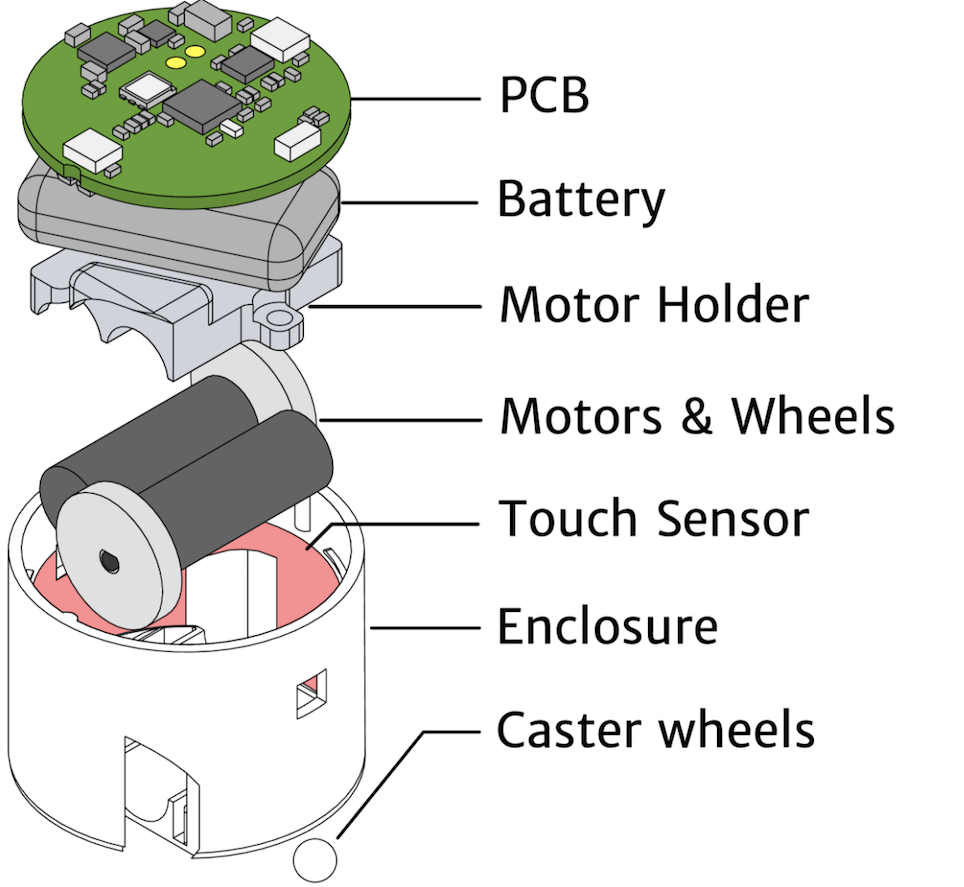
\includegraphics[height=10cm]{Zooids.png}
    \caption{Zooids}
    \label{fig:Zooids}
\end{figure}

\begin{figure}[htbp]
    \centering
    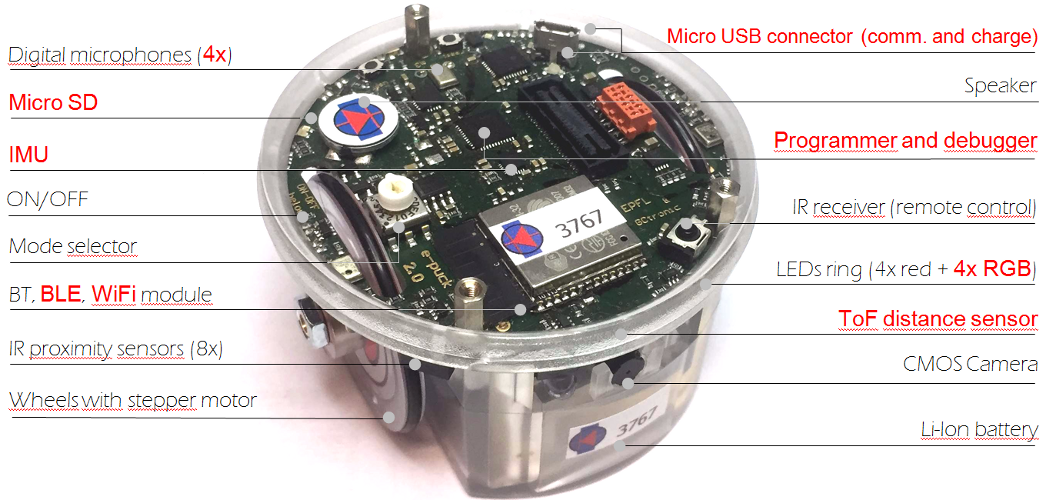
\includegraphics[height=6cm]{e-puck2-features_small.png}
    \caption{Zooids}
    \label{fig:e-puck}
\end{figure}

\begin{figure}[htbp]
    \centering
    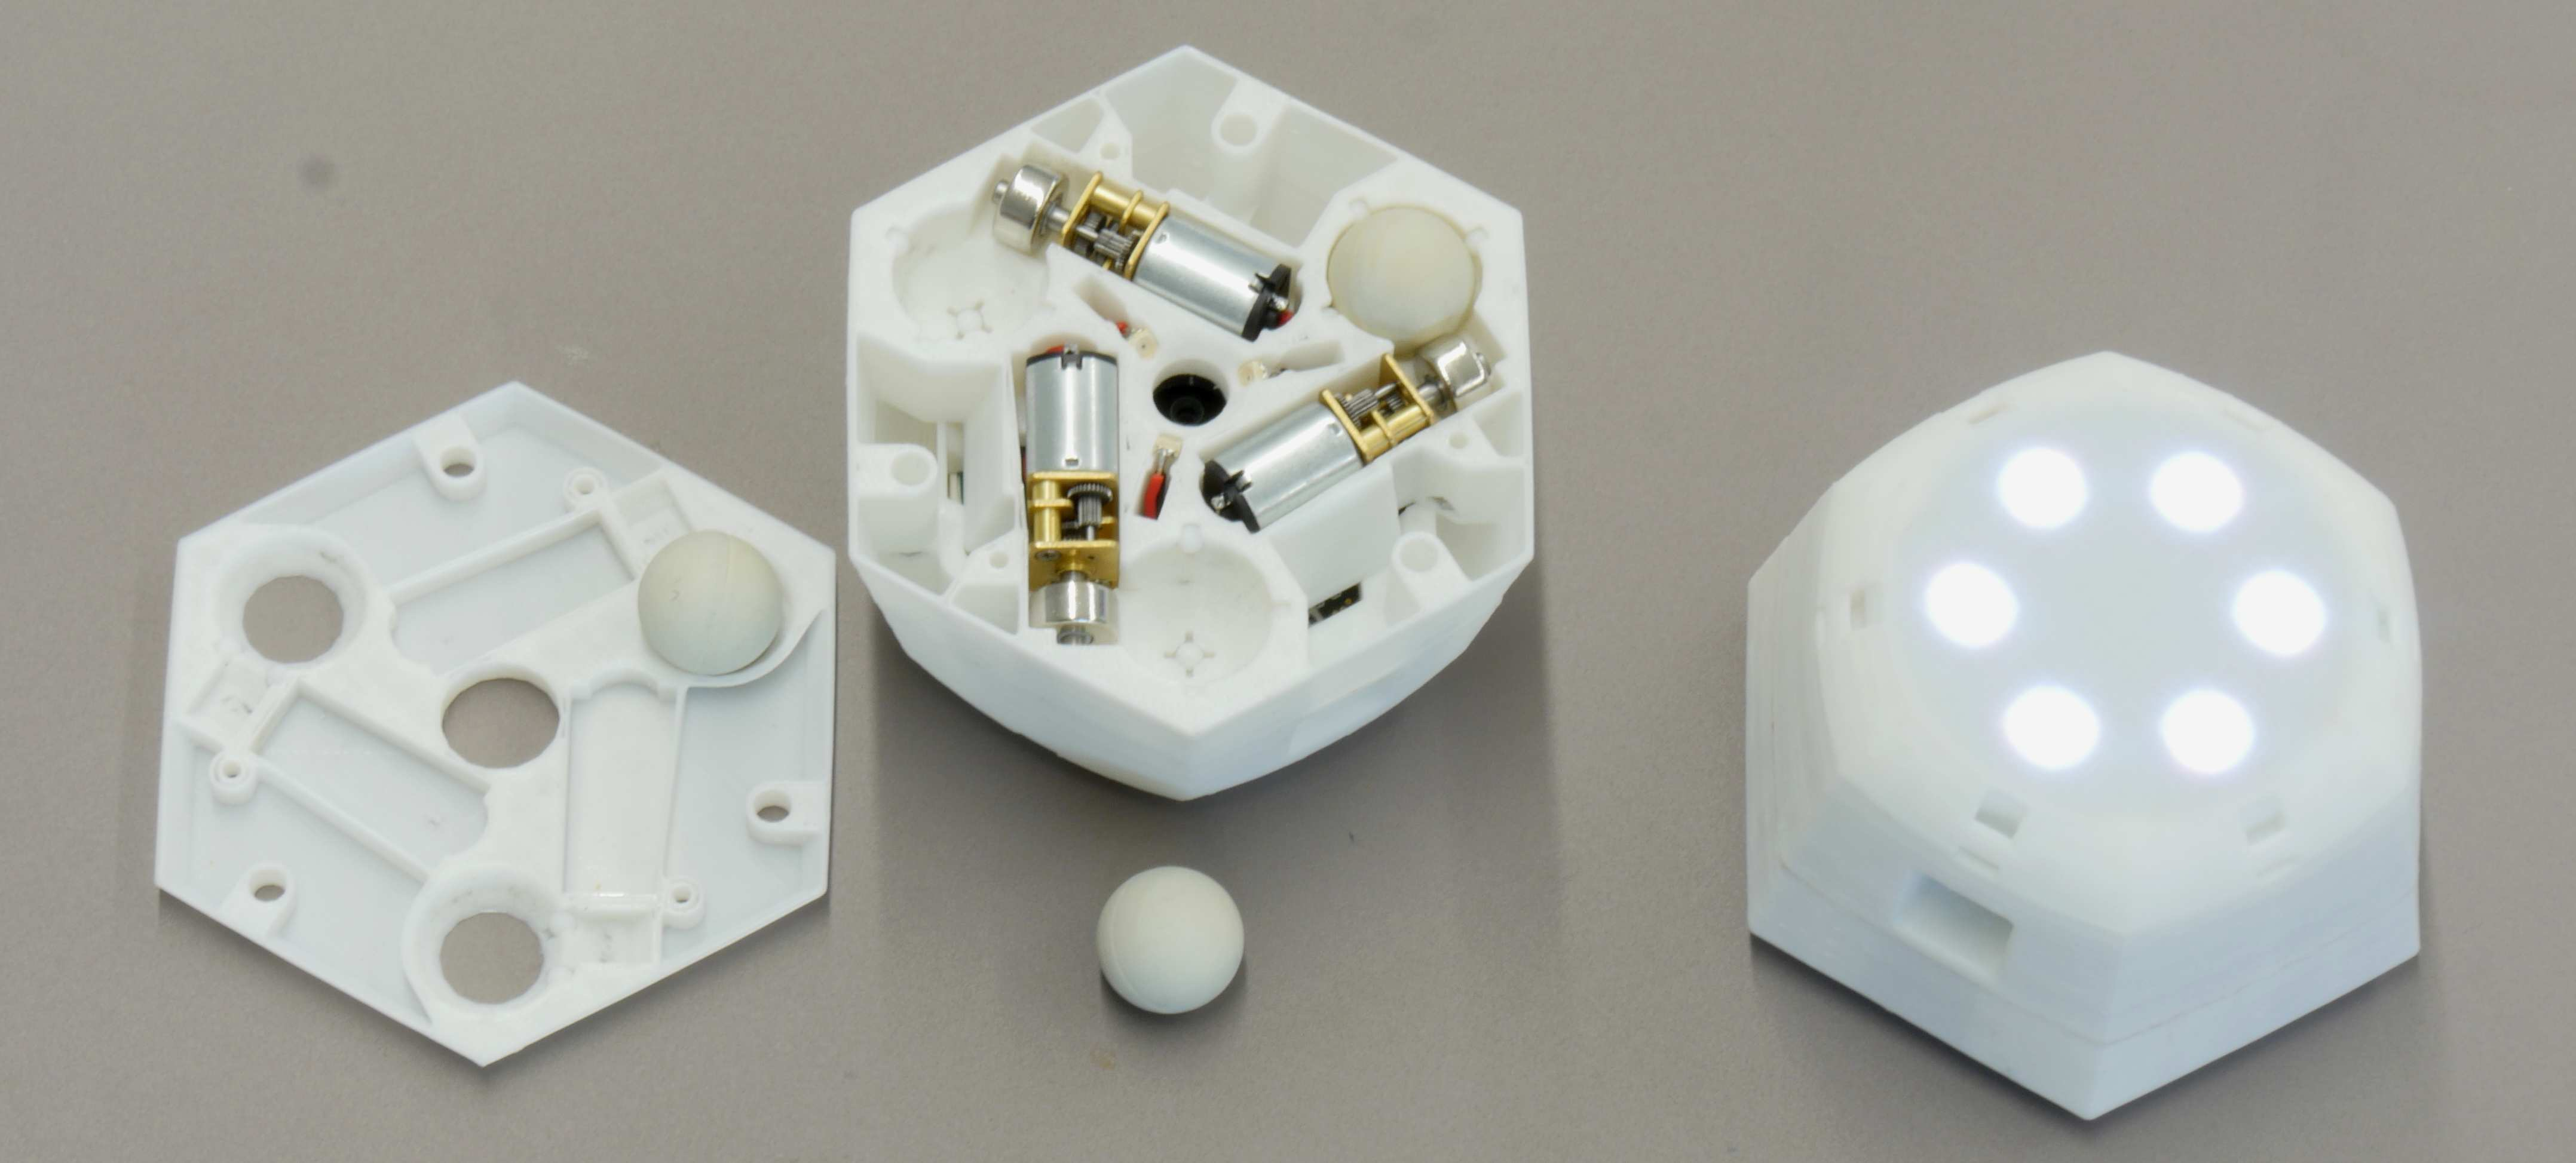
\includegraphics[height=6cm]{cellulo.jpg}
    \caption{Cellulo}
    \label{fig:Cellulo}
\end{figure}
  
\begin{figure}[htbp]
    \centering
    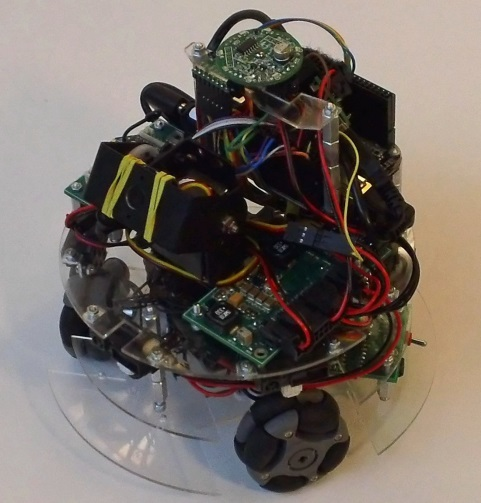
\includegraphics[height=10cm]{WolfBot.jpg}
    \caption{WolfBot}
    \label{fig:WolfBot}
\end{figure}

经过尝试,我们发现磁驱电机的速度和磁环的磁性强弱、电池的电量剩余、磁环和轴之间的胶合强度等不可控因素关系很大,无法建立起小车各轮速度和电机PWM占空比之间的时不变映射关系,导致很难控制小车的走向和速度,最终放弃了这一想法。

WolfBot采用的全向轮和电机直接连接,使得底盘占地面积很大。最终我们则采用1.5英寸麦克纳姆轮和GW12-N20减速电机(减速齿轮中的蜗杆改变90度传动方向)实现系统最小化。

\section{三轮全向轮移动平台}

经典的三轮全向轮(Omni Wheel)移动平台全向轮中心平均分布在一个圆上。

\begin{equation}
    \left[\begin{array}{l}
    {V_{1}} \\
    {V_{2}} \\
    {V_{3}}
    \end{array}\right]=\left[\begin{array}{ccc}
    {-1} & {0} & {L} \\
    {\sin \frac{\pi}{6}} & {-\cos \frac{\pi}{6}} & {L} \\
    {\sin \frac{\pi}{6}} & {\cos \frac{\pi}{6}} & {L}
    \end{array}\right]\left[\begin{array}{l}
    {V_{x}} \\
    {V_{y}} \\
    {\omega}
    \end{array}\right]
\end{equation}

解算可得V1、V2、V3表达式:

\begin{equation}
    \left\{\begin{aligned}
    &V_{1}=-\frac{1}{2} V_{x}+\frac{\sqrt{3}}{2} V_{y}+L \omega \\
    &V_{2}=-\frac{1}{2} V_{x}-\frac{\sqrt{3}}{2} V_{y}+L \omega \\
    &V_{3}=V_{x}+L \omega
    \end{aligned}\right.
\end{equation}

\section{麦克纳姆轮}

\subsection{Mecanum wheel简介}
当需要车辆全向运动时,可以使用麦克纳姆轮(Mecanum wheel),如图~\ref{fig:Mecanum-wheel}。车辆可以沿着规定的路径移动,并同时绕其中心任意旋转,如图~\ref{fig:Vehicle-with-3-Mecanum-wheels}。麦克纳努姆轮由围绕轮轴排列的一组辊(roller)组成。

\begin{figure}
    \begin{minipage}{0.48\textwidth}
      \centering
      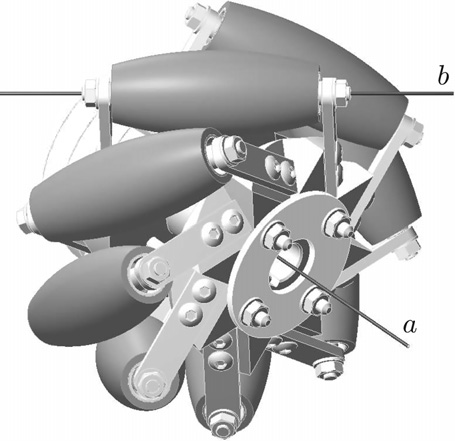
\includegraphics[height=5cm]{Mecanum-wheel.jpg}
      \caption{麦克纳姆轮}
      \label{fig:Mecanum-wheel}
    \end{minipage}\hfill
    \begin{minipage}{0.48\textwidth}
      \centering
      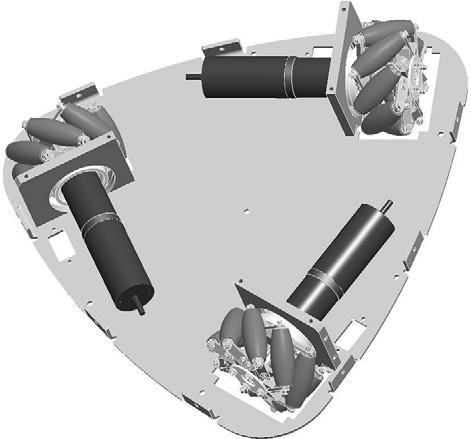
\includegraphics[height=5cm]{Vehicle-with-3-Mecanum-wheels.jpg}
      \caption{3麦克纳姆轮小车}
      \label{fig:Vehicle-with-3-Mecanum-wheels}
    \end{minipage}
\end{figure}

\subsection{Mecanum wheel几何描述}
为了使麦克纳姆轮能够在任意时刻都至少有一个辊子紧密接触地面,其几何学描述见图~\ref{fig:Curve-cR-generating-the-rolls}和图~\ref{fig:The-roll-surface-R},推导见Geometry and kinematics of the Mecanum wheel\cite{gfrerrer2008geometry}一文。

\begin{figure}[htbp]
    \centering
    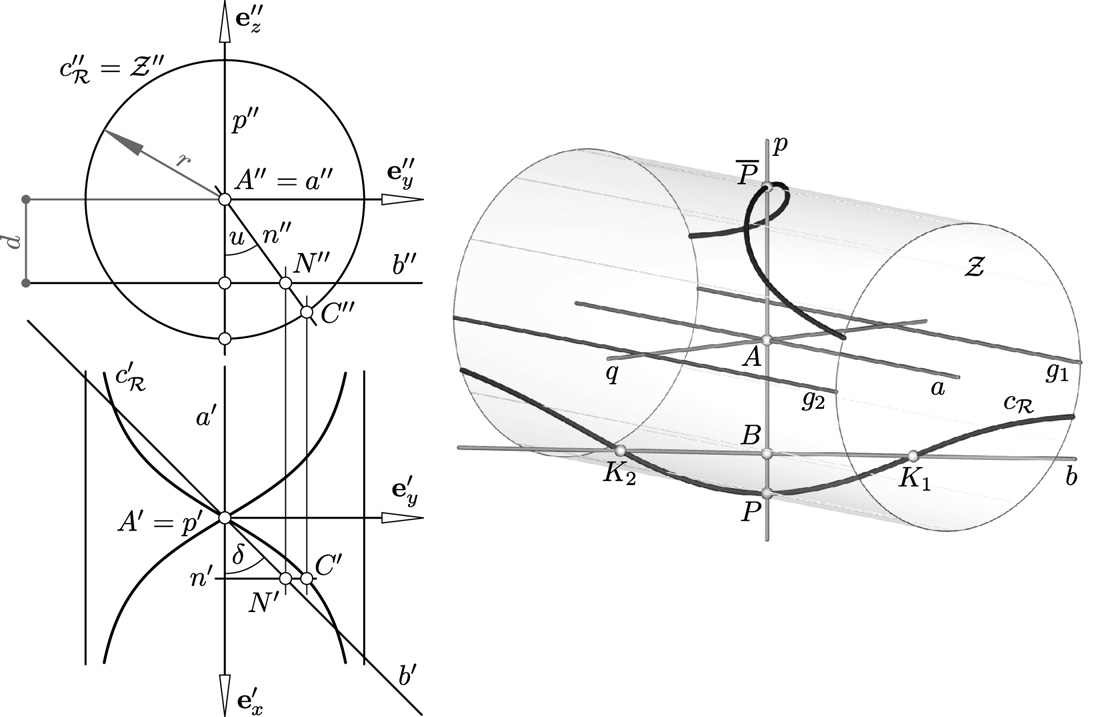
\includegraphics[height=10cm]{Curve-cR-generating-the-rolls.jpg}
    \caption{生成辊子曲面的曲线cR}
    \label{fig:Curve-cR-generating-the-rolls}
\end{figure}

\begin{figure}[htbp]
    \centering
    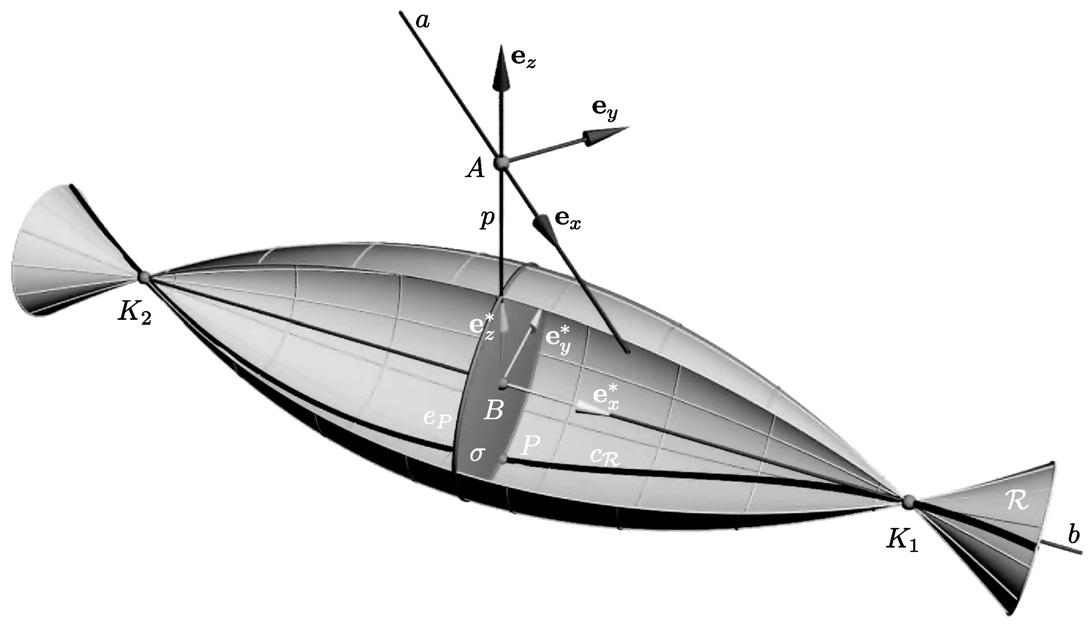
\includegraphics[height=8cm]{The-roll-surface-R.jpg}
    \caption{辊子曲面R}
    \label{fig:The-roll-surface-R}
\end{figure}

\subsection{Mecanum wheel动力学模型}


\subsection{三麦克纳姆轮系统运动控制}

\section{主控板}

\section{扩展接口}

\section{实物可视化界面}

\section{UI}